% Options for packages loaded elsewhere
\PassOptionsToPackage{unicode}{hyperref}
\PassOptionsToPackage{hyphens}{url}
%
\documentclass[
]{article}
\usepackage{lmodern}
\usepackage{amssymb,amsmath}
\usepackage{ifxetex,ifluatex}
\ifnum 0\ifxetex 1\fi\ifluatex 1\fi=0 % if pdftex
  \usepackage[T1]{fontenc}
  \usepackage[utf8]{inputenc}
  \usepackage{textcomp} % provide euro and other symbols
\else % if luatex or xetex
  \usepackage{unicode-math}
  \defaultfontfeatures{Scale=MatchLowercase}
  \defaultfontfeatures[\rmfamily]{Ligatures=TeX,Scale=1}
\fi
% Use upquote if available, for straight quotes in verbatim environments
\IfFileExists{upquote.sty}{\usepackage{upquote}}{}
\IfFileExists{microtype.sty}{% use microtype if available
  \usepackage[]{microtype}
  \UseMicrotypeSet[protrusion]{basicmath} % disable protrusion for tt fonts
}{}
\makeatletter
\@ifundefined{KOMAClassName}{% if non-KOMA class
  \IfFileExists{parskip.sty}{%
    \usepackage{parskip}
  }{% else
    \setlength{\parindent}{0pt}
    \setlength{\parskip}{6pt plus 2pt minus 1pt}}
}{% if KOMA class
  \KOMAoptions{parskip=half}}
\makeatother
\usepackage{xcolor}
\IfFileExists{xurl.sty}{\usepackage{xurl}}{} % add URL line breaks if available
\IfFileExists{bookmark.sty}{\usepackage{bookmark}}{\usepackage{hyperref}}
\hypersetup{
  pdfauthor={Xwyzworm},
  hidelinks,
  pdfcreator={LaTeX via pandoc}}
\urlstyle{same} % disable monospaced font for URLs
\usepackage[margin=1in]{geometry}
\usepackage{color}
\usepackage{fancyvrb}
\newcommand{\VerbBar}{|}
\newcommand{\VERB}{\Verb[commandchars=\\\{\}]}
\DefineVerbatimEnvironment{Highlighting}{Verbatim}{commandchars=\\\{\}}
% Add ',fontsize=\small' for more characters per line
\usepackage{framed}
\definecolor{shadecolor}{RGB}{248,248,248}
\newenvironment{Shaded}{\begin{snugshade}}{\end{snugshade}}
\newcommand{\AlertTok}[1]{\textcolor[rgb]{0.94,0.16,0.16}{#1}}
\newcommand{\AnnotationTok}[1]{\textcolor[rgb]{0.56,0.35,0.01}{\textbf{\textit{#1}}}}
\newcommand{\AttributeTok}[1]{\textcolor[rgb]{0.77,0.63,0.00}{#1}}
\newcommand{\BaseNTok}[1]{\textcolor[rgb]{0.00,0.00,0.81}{#1}}
\newcommand{\BuiltInTok}[1]{#1}
\newcommand{\CharTok}[1]{\textcolor[rgb]{0.31,0.60,0.02}{#1}}
\newcommand{\CommentTok}[1]{\textcolor[rgb]{0.56,0.35,0.01}{\textit{#1}}}
\newcommand{\CommentVarTok}[1]{\textcolor[rgb]{0.56,0.35,0.01}{\textbf{\textit{#1}}}}
\newcommand{\ConstantTok}[1]{\textcolor[rgb]{0.00,0.00,0.00}{#1}}
\newcommand{\ControlFlowTok}[1]{\textcolor[rgb]{0.13,0.29,0.53}{\textbf{#1}}}
\newcommand{\DataTypeTok}[1]{\textcolor[rgb]{0.13,0.29,0.53}{#1}}
\newcommand{\DecValTok}[1]{\textcolor[rgb]{0.00,0.00,0.81}{#1}}
\newcommand{\DocumentationTok}[1]{\textcolor[rgb]{0.56,0.35,0.01}{\textbf{\textit{#1}}}}
\newcommand{\ErrorTok}[1]{\textcolor[rgb]{0.64,0.00,0.00}{\textbf{#1}}}
\newcommand{\ExtensionTok}[1]{#1}
\newcommand{\FloatTok}[1]{\textcolor[rgb]{0.00,0.00,0.81}{#1}}
\newcommand{\FunctionTok}[1]{\textcolor[rgb]{0.00,0.00,0.00}{#1}}
\newcommand{\ImportTok}[1]{#1}
\newcommand{\InformationTok}[1]{\textcolor[rgb]{0.56,0.35,0.01}{\textbf{\textit{#1}}}}
\newcommand{\KeywordTok}[1]{\textcolor[rgb]{0.13,0.29,0.53}{\textbf{#1}}}
\newcommand{\NormalTok}[1]{#1}
\newcommand{\OperatorTok}[1]{\textcolor[rgb]{0.81,0.36,0.00}{\textbf{#1}}}
\newcommand{\OtherTok}[1]{\textcolor[rgb]{0.56,0.35,0.01}{#1}}
\newcommand{\PreprocessorTok}[1]{\textcolor[rgb]{0.56,0.35,0.01}{\textit{#1}}}
\newcommand{\RegionMarkerTok}[1]{#1}
\newcommand{\SpecialCharTok}[1]{\textcolor[rgb]{0.00,0.00,0.00}{#1}}
\newcommand{\SpecialStringTok}[1]{\textcolor[rgb]{0.31,0.60,0.02}{#1}}
\newcommand{\StringTok}[1]{\textcolor[rgb]{0.31,0.60,0.02}{#1}}
\newcommand{\VariableTok}[1]{\textcolor[rgb]{0.00,0.00,0.00}{#1}}
\newcommand{\VerbatimStringTok}[1]{\textcolor[rgb]{0.31,0.60,0.02}{#1}}
\newcommand{\WarningTok}[1]{\textcolor[rgb]{0.56,0.35,0.01}{\textbf{\textit{#1}}}}
\usepackage{graphicx,grffile}
\makeatletter
\def\maxwidth{\ifdim\Gin@nat@width>\linewidth\linewidth\else\Gin@nat@width\fi}
\def\maxheight{\ifdim\Gin@nat@height>\textheight\textheight\else\Gin@nat@height\fi}
\makeatother
% Scale images if necessary, so that they will not overflow the page
% margins by default, and it is still possible to overwrite the defaults
% using explicit options in \includegraphics[width, height, ...]{}
\setkeys{Gin}{width=\maxwidth,height=\maxheight,keepaspectratio}
% Set default figure placement to htbp
\makeatletter
\def\fps@figure{htbp}
\makeatother
\setlength{\emergencystretch}{3em} % prevent overfull lines
\providecommand{\tightlist}{%
  \setlength{\itemsep}{0pt}\setlength{\parskip}{0pt}}
\setcounter{secnumdepth}{-\maxdimen} % remove section numbering

\author{Xwyzworm}
\date{}

\begin{document}

\hypertarget{introduction}{%
\subsection{Introduction :}\label{introduction}}

The goal of the assignment is to explore the NOAA Storm Database and
explore the effects of severe weather events on both population and
economy.The database covers the time period between 1950 and November
2011.

The following analysis investigates which types of severe Disasters are
most harmful on:

Health (injuries and fatalities) Property and crops (economic
consequences) \#\# My Software Environment

\begin{Shaded}
\begin{Highlighting}[]
\KeywordTok{sessionInfo}\NormalTok{()}
\end{Highlighting}
\end{Shaded}

\begin{verbatim}
## R version 4.0.1 (2020-06-06)
## Platform: x86_64-w64-mingw32/x64 (64-bit)
## Running under: Windows 10 x64 (build 18363)
## 
## Matrix products: default
## 
## locale:
## [1] LC_COLLATE=English_Indonesia.1252  LC_CTYPE=English_Indonesia.1252   
## [3] LC_MONETARY=English_Indonesia.1252 LC_NUMERIC=C                      
## [5] LC_TIME=English_Indonesia.1252    
## 
## attached base packages:
## [1] stats     graphics  grDevices utils     datasets  methods   base     
## 
## loaded via a namespace (and not attached):
##  [1] compiler_4.0.1  magrittr_1.5    tools_4.0.1     htmltools_0.4.0
##  [5] yaml_2.2.1      Rcpp_1.0.4.6    stringi_1.4.6   rmarkdown_2.2  
##  [9] knitr_1.28      stringr_1.4.0   xfun_0.14       digest_0.6.25  
## [13] rlang_0.4.6     evaluate_0.14
\end{verbatim}

\hypertarget{data-processing}{%
\subsection{Data Processing}\label{data-processing}}

\hypertarget{loading-reading-data}{%
\subsubsection{Loading \& reading data}\label{loading-reading-data}}

\begin{Shaded}
\begin{Highlighting}[]
\KeywordTok{library}\NormalTok{(dplyr)}
\end{Highlighting}
\end{Shaded}

\begin{verbatim}
## 
## Attaching package: 'dplyr'
\end{verbatim}

\begin{verbatim}
## The following objects are masked from 'package:stats':
## 
##     filter, lag
\end{verbatim}

\begin{verbatim}
## The following objects are masked from 'package:base':
## 
##     intersect, setdiff, setequal, union
\end{verbatim}

\begin{Shaded}
\begin{Highlighting}[]
\KeywordTok{library}\NormalTok{(plyr)}
\end{Highlighting}
\end{Shaded}

\begin{verbatim}
## Warning: package 'plyr' was built under R version 4.0.2
\end{verbatim}

\begin{verbatim}
## ------------------------------------------------------------------------------
\end{verbatim}

\begin{verbatim}
## You have loaded plyr after dplyr - this is likely to cause problems.
## If you need functions from both plyr and dplyr, please load plyr first, then dplyr:
## library(plyr); library(dplyr)
\end{verbatim}

\begin{verbatim}
## ------------------------------------------------------------------------------
\end{verbatim}

\begin{verbatim}
## 
## Attaching package: 'plyr'
\end{verbatim}

\begin{verbatim}
## The following objects are masked from 'package:dplyr':
## 
##     arrange, count, desc, failwith, id, mutate, rename, summarise,
##     summarize
\end{verbatim}

\begin{Shaded}
\begin{Highlighting}[]
\KeywordTok{library}\NormalTok{(ggplot2) }
\KeywordTok{library}\NormalTok{(reshape2) }
\end{Highlighting}
\end{Shaded}

\begin{verbatim}
## Warning: package 'reshape2' was built under R version 4.0.2
\end{verbatim}

\begin{Shaded}
\begin{Highlighting}[]
\KeywordTok{setwd}\NormalTok{(}\StringTok{"D:/Reproducible Research/Week4"}\NormalTok{)}
\CommentTok{#fileurl <- "https://d396qusza40orc.cloudfront.net/repdata%2Fdata%2FStormData.csv.bz2"}
\CommentTok{#download.file(url = fileurl , destfile = "DataSet/repdata_data_StormData.csv")}

\NormalTok{stromdf <-}\StringTok{ }\KeywordTok{read.csv}\NormalTok{(}\StringTok{"./DataSet/repdata_data_StormData.csv/repdata_data_StormData.csv"}\NormalTok{)}
\NormalTok{stromdf <-}\StringTok{ }\NormalTok{stromdf[,}\KeywordTok{c}\NormalTok{(}\StringTok{"EVTYPE"}\NormalTok{ , }\StringTok{"FATALITIES"}\NormalTok{,}\StringTok{"INJURIES"}\NormalTok{,}\StringTok{"PROPDMG"}\NormalTok{,}\StringTok{"PROPDMGEXP"}\NormalTok{,}\StringTok{"CROPDMG"}\NormalTok{,}\StringTok{"CROPDMGEXP"}\NormalTok{)]}
\end{Highlighting}
\end{Shaded}

\hypertarget{subsetting-preprocessing-data}{%
\subsubsection{Subsetting \& Preprocessing
Data}\label{subsetting-preprocessing-data}}

This is important because there's alot things to be done , data is messy

\begin{Shaded}
\begin{Highlighting}[]
\NormalTok{TotalGrouped <-}\StringTok{ }\KeywordTok{subset}\NormalTok{(stromdf , EVTYPE }\OperatorTok{!=}\StringTok{ '?'} \OperatorTok{&}\StringTok{ }\NormalTok{(FATALITIES }\OperatorTok{>}\StringTok{ }\DecValTok{0} \OperatorTok{|}\StringTok{ }\NormalTok{INJURIES }\OperatorTok{>}\StringTok{ }\DecValTok{0} \OperatorTok{|}\StringTok{ }\NormalTok{PROPDMG }\OperatorTok{>}\StringTok{ }\DecValTok{0} \OperatorTok{|}\StringTok{ }\NormalTok{CROPDMG }\OperatorTok{>}\StringTok{ }\DecValTok{0}\NormalTok{))}

\NormalTok{TotalGrouped}\OperatorTok{$}\NormalTok{PROPDMGEXP <-}\StringTok{ }\KeywordTok{toupper}\NormalTok{(TotalGrouped}\OperatorTok{$}\NormalTok{PROPDMGEXP)}
\NormalTok{TotalGrouped}\OperatorTok{$}\NormalTok{CROPDMGEXP <-}\StringTok{ }\KeywordTok{toupper}\NormalTok{(TotalGrouped}\OperatorTok{$}\NormalTok{CROPDMGEXP)}
\CommentTok{## Convert the Exponent Variables}
\NormalTok{Propdmgconv <-}\StringTok{ }\KeywordTok{c}\NormalTok{(}\StringTok{"-"}\NormalTok{ =}\StringTok{ }\DecValTok{10}\OperatorTok{^}\DecValTok{0}\NormalTok{, }\StringTok{"+"}\NormalTok{ =}\StringTok{ }\DecValTok{10}\OperatorTok{^}\DecValTok{0}\NormalTok{,}
                 \StringTok{"H"}\NormalTok{ =}\StringTok{ }\DecValTok{10}\OperatorTok{^}\DecValTok{2}\NormalTok{, }\StringTok{"K"}\NormalTok{ =}\StringTok{ }\DecValTok{10}\OperatorTok{^}\DecValTok{3}\NormalTok{,}
                 \StringTok{"M"}\NormalTok{ =}\StringTok{ }\DecValTok{10}\OperatorTok{^}\DecValTok{6}\NormalTok{, }\StringTok{"B"}\NormalTok{ =}\StringTok{ }\DecValTok{10}\OperatorTok{^}\DecValTok{9}\NormalTok{,}
                 \StringTok{"0"}\NormalTok{ =}\StringTok{ }\DecValTok{10}\OperatorTok{^}\DecValTok{0}\NormalTok{, }\StringTok{"1"}\NormalTok{ =}\StringTok{ }\DecValTok{10}\OperatorTok{^}\DecValTok{1}\NormalTok{,}
                 \StringTok{"2"}\NormalTok{ =}\StringTok{ }\DecValTok{10}\OperatorTok{^}\DecValTok{2}\NormalTok{, }\StringTok{"3"}\NormalTok{ =}\StringTok{ }\DecValTok{10}\OperatorTok{^}\DecValTok{3}\NormalTok{,}
                 \StringTok{"4"}\NormalTok{ =}\StringTok{ }\DecValTok{10}\OperatorTok{^}\DecValTok{4}\NormalTok{, }\StringTok{"5"}\NormalTok{ =}\StringTok{ }\DecValTok{10}\OperatorTok{^}\DecValTok{5}\NormalTok{,}
                 \StringTok{"6"}\NormalTok{ =}\StringTok{ }\DecValTok{10}\OperatorTok{^}\DecValTok{6}\NormalTok{, }\StringTok{"7"}\NormalTok{ =}\StringTok{ }\DecValTok{10}\OperatorTok{^}\DecValTok{7}\NormalTok{,}
                 \StringTok{"8"}\NormalTok{ =}\StringTok{ }\DecValTok{10}\OperatorTok{^}\DecValTok{8}\NormalTok{ ,}\StringTok{"9"}\NormalTok{ =}\StringTok{ }\DecValTok{10}\OperatorTok{^}\DecValTok{9}\NormalTok{)}
\NormalTok{Cropdmgconv <-}\StringTok{ }\KeywordTok{c}\NormalTok{( }
                 \StringTok{"?"}\NormalTok{ =}\StringTok{ }\DecValTok{10}\OperatorTok{^}\DecValTok{0}\NormalTok{,}\StringTok{"0"}\NormalTok{ =}\StringTok{ }\DecValTok{10}\OperatorTok{^}\DecValTok{0}\NormalTok{,}
                 \StringTok{"K"}\NormalTok{ =}\StringTok{ }\DecValTok{10}\OperatorTok{^}\DecValTok{3}\NormalTok{,}\StringTok{"M"}\NormalTok{ =}\StringTok{ }\DecValTok{10}\OperatorTok{^}\DecValTok{4}\NormalTok{,}
                 \StringTok{"B"}\NormalTok{ =}\StringTok{ }\DecValTok{10}\OperatorTok{^}\DecValTok{9}\NormalTok{) }
\NormalTok{TotalGrouped}\OperatorTok{$}\NormalTok{PROPDMGEXP[TotalGrouped}\OperatorTok{$}\NormalTok{PROPDMGEXP }\OperatorTok{==}\StringTok{ ""}\NormalTok{] <-}\StringTok{ }\DecValTok{10}\OperatorTok{^}\DecValTok{0}
\NormalTok{TotalGrouped}\OperatorTok{$}\NormalTok{CROPDMGEXP[TotalGrouped}\OperatorTok{$}\NormalTok{CROPDMGEXP }\OperatorTok{==}\StringTok{ ""}\NormalTok{] <-}\StringTok{ }\DecValTok{10}\OperatorTok{^}\DecValTok{0}

\NormalTok{TotalGrouped}\OperatorTok{$}\NormalTok{PROPDMGEXP <-}\StringTok{ }\KeywordTok{revalue}\NormalTok{(TotalGrouped}\OperatorTok{$}\NormalTok{PROPDMGEXP , Propdmgconv)}
\end{Highlighting}
\end{Shaded}

\begin{verbatim}
## The following `from` values were not present in `x`: 8, 9
\end{verbatim}

\begin{Shaded}
\begin{Highlighting}[]
\NormalTok{TotalGrouped}\OperatorTok{$}\NormalTok{CROPDMGEXP <-}\StringTok{ }\KeywordTok{revalue}\NormalTok{(TotalGrouped}\OperatorTok{$}\NormalTok{CROPDMGEXP , Cropdmgconv)}
\end{Highlighting}
\end{Shaded}

\hypertarget{calculate-total-fatalities-and-injuries-then-melt-the-top10}{%
\subsubsection{Calculate Total Fatalities and Injuries then Melt the
top10}\label{calculate-total-fatalities-and-injuries-then-melt-the-top10}}

\begin{Shaded}
\begin{Highlighting}[]
\NormalTok{TotalGrouped }\OperatorTok\StringTok{ }
\StringTok{        }\NormalTok{dplyr}\OperatorTok{::}\KeywordTok{group_by}\NormalTok{(EVTYPE) }\OperatorTok
\StringTok{        }\NormalTok{dplyr}\OperatorTok{::}\KeywordTok{summarise}\NormalTok{(}\DataTypeTok{FATALITIES =} \KeywordTok{sum}\NormalTok{(FATALITIES),}\DataTypeTok{INJURIES =} \KeywordTok{sum}\NormalTok{(INJURIES),}
                         \DataTypeTok{TOTAL =} \KeywordTok{sum}\NormalTok{(FATALITIES) }\OperatorTok{+}\StringTok{ }\KeywordTok{sum}\NormalTok{(INJURIES)) ->}\StringTok{ }\NormalTok{Totalaccident}
\end{Highlighting}
\end{Shaded}

\begin{verbatim}
## `summarise()` ungrouping output (override with `.groups` argument)
\end{verbatim}

\begin{Shaded}
\begin{Highlighting}[]
\NormalTok{Totalaccident <-}\StringTok{ }\NormalTok{Totalaccident[}\KeywordTok{order}\NormalTok{(}\OperatorTok{-}\NormalTok{Totalaccident}\OperatorTok{$}\NormalTok{FATALITIES),] }\CommentTok{# Sorting Values}
\NormalTok{Top10 <-}\StringTok{ }\KeywordTok{head}\NormalTok{(Totalaccident , }\DataTypeTok{n =}\DecValTok{10}\NormalTok{)}
\NormalTok{Top10 <-}\StringTok{ }\NormalTok{reshape2}\OperatorTok{::}\KeywordTok{melt}\NormalTok{(}\DataTypeTok{data =}\NormalTok{ Top10 , }\DataTypeTok{id.vars =} \KeywordTok{c}\NormalTok{(}\StringTok{"EVTYPE"}\NormalTok{) ,}\DataTypeTok{variable.name =} \StringTok{"accident"}\NormalTok{)}
\end{Highlighting}
\end{Shaded}

\hypertarget{plot-the-top-10-dangerous-disasters}{%
\subsubsection{Plot The top 10 Dangerous
Disasters}\label{plot-the-top-10-dangerous-disasters}}

\begin{Shaded}
\begin{Highlighting}[]
\NormalTok{ggplot2}\OperatorTok{::}\KeywordTok{ggplot}\NormalTok{(}\DataTypeTok{data =}\NormalTok{ Top10, }\KeywordTok{aes}\NormalTok{(}\DataTypeTok{x =} \KeywordTok{reorder}\NormalTok{(EVTYPE, }\OperatorTok{-}\NormalTok{value) , }\DataTypeTok{y =}\NormalTok{ value , }\DataTypeTok{fill =}\NormalTok{ accident)) }\OperatorTok{+}
\StringTok{        }\NormalTok{ggplot2}\OperatorTok{::}\KeywordTok{geom_bar}\NormalTok{(}\DataTypeTok{stat =} \StringTok{"identity"}\NormalTok{ , }\DataTypeTok{position =} \StringTok{'dodge'}\NormalTok{) }\OperatorTok{+}
\StringTok{        }\NormalTok{ggplot2}\OperatorTok{::}\KeywordTok{labs}\NormalTok{(}\DataTypeTok{x =} \StringTok{"Disasters"}\NormalTok{ , }\DataTypeTok{y =} \StringTok{"Total Value"}\NormalTok{ , }\DataTypeTok{title =} \StringTok{"Top 10 Disasters causing Death"}\NormalTok{) }\OperatorTok{+}
\StringTok{        }\NormalTok{ggplot2}\OperatorTok{::}\KeywordTok{theme}\NormalTok{(}\DataTypeTok{axis.text.x =} \KeywordTok{element_text}\NormalTok{(}\DataTypeTok{angle =} \DecValTok{45}\NormalTok{ ,}\DataTypeTok{size =} \DecValTok{7}\NormalTok{)) }
\end{Highlighting}
\end{Shaded}

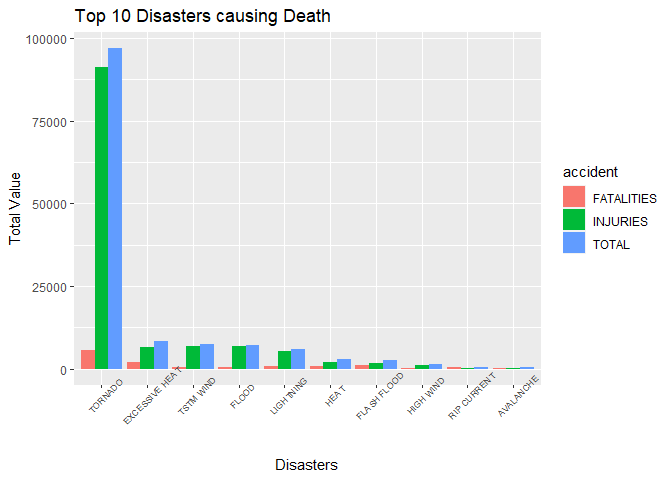
\includegraphics{FinalScript_files/figure-latex/unnamed-chunk-5-1.pdf}
So From here we know that tornado make people get injuried the
most,compare others.

\hypertarget{economic-consiquencies}{%
\subsubsection{Economic Consiquencies}\label{economic-consiquencies}}

\hypertarget{calculate-total-prop-crop-loss-then-melt-it.}{%
\subsubsection{Calculate Total Prop \& Crop Loss Then Melt
it.}\label{calculate-total-prop-crop-loss-then-melt-it.}}

\begin{Shaded}
\begin{Highlighting}[]
\NormalTok{OverallLoss <-}\StringTok{ }\NormalTok{TotalGrouped}

\NormalTok{OverallLoss}\OperatorTok{$}\NormalTok{proploss <-}\StringTok{ }\NormalTok{OverallLoss}\OperatorTok{$}\NormalTok{PROPDMG }\OperatorTok{*}\StringTok{ }\KeywordTok{as.numeric}\NormalTok{(OverallLoss}\OperatorTok{$}\NormalTok{PROPDMGEXP)}
\NormalTok{OverallLoss}\OperatorTok{$}\NormalTok{croploss <-}\StringTok{ }\NormalTok{OverallLoss}\OperatorTok{$}\NormalTok{CROPDMG }\OperatorTok{*}\StringTok{ }\KeywordTok{as.numeric}\NormalTok{(OverallLoss}\OperatorTok{$}\NormalTok{CROPDMGEXP)}

\NormalTok{OverallLoss }\OperatorTok\StringTok{ }
\StringTok{        }\NormalTok{dplyr}\OperatorTok{::}\KeywordTok{group_by}\NormalTok{(EVTYPE) }\OperatorTok
\StringTok{        }\NormalTok{dplyr}\OperatorTok{::}\KeywordTok{summarise}\NormalTok{(}\DataTypeTok{proplossTot =} \KeywordTok{sum}\NormalTok{(proploss) ,}
                  \DataTypeTok{CROPlossTot =} \KeywordTok{sum}\NormalTok{(croploss) , }
                  \DataTypeTok{TotalLoss =} \KeywordTok{sum}\NormalTok{(proplossTot) }\OperatorTok{+}\StringTok{ }\KeywordTok{sum}\NormalTok{(CROPlossTot))  ->}\StringTok{ }\NormalTok{OverallLoss}
\end{Highlighting}
\end{Shaded}

\begin{verbatim}
## `summarise()` ungrouping output (override with `.groups` argument)
\end{verbatim}

\begin{Shaded}
\begin{Highlighting}[]
\NormalTok{OverallLoss <-}\StringTok{ }\NormalTok{OverallLoss[}\KeywordTok{order}\NormalTok{(}\OperatorTok{-}\NormalTok{OverallLoss}\OperatorTok{$}\NormalTok{TotalLoss) , ] }
\NormalTok{Top10Loss <-}\StringTok{ }\KeywordTok{head}\NormalTok{(OverallLoss , }\DecValTok{10}\NormalTok{)}
\NormalTok{Top10Loss <-reshape2}\OperatorTok{::}\KeywordTok{melt}\NormalTok{(}\DataTypeTok{data =}\NormalTok{ Top10Loss , }\DataTypeTok{id.vars =} \KeywordTok{c}\NormalTok{(}\StringTok{'EVTYPE'}\NormalTok{),}\DataTypeTok{variable.name =} \StringTok{"Disasters"}\NormalTok{)}
\end{Highlighting}
\end{Shaded}

\hypertarget{plot-the-top-10-dangerous-disasters-for-economic}{%
\subsubsection{Plot The Top 10 Dangerous Disasters for
Economic}\label{plot-the-top-10-dangerous-disasters-for-economic}}

\begin{Shaded}
\begin{Highlighting}[]
\NormalTok{ggplot2}\OperatorTok{::}\KeywordTok{ggplot}\NormalTok{(}\DataTypeTok{data =}\NormalTok{ Top10Loss , }\KeywordTok{aes}\NormalTok{(}\DataTypeTok{x =} \KeywordTok{reorder}\NormalTok{(EVTYPE , }\OperatorTok{-}\NormalTok{value) , }\DataTypeTok{y =}\NormalTok{value ,}\DataTypeTok{fill =}\NormalTok{ Disasters )) }\OperatorTok{+}
\StringTok{        }\NormalTok{ggplot2}\OperatorTok{::}\KeywordTok{geom_bar}\NormalTok{(}\DataTypeTok{stat =} \StringTok{"identity"}\NormalTok{ , }\DataTypeTok{position =} \StringTok{"dodge"}\NormalTok{ ,) }\OperatorTok{+}\StringTok{ }
\StringTok{        }\NormalTok{ggplot2}\OperatorTok{::}\KeywordTok{labs}\NormalTok{(}\DataTypeTok{x =} \StringTok{"Disasters"}\NormalTok{ , }\DataTypeTok{y =} \StringTok{"Total Value"}\NormalTok{ , }\DataTypeTok{title =} \StringTok{"Top 10 Disasters causing Big Loss"}\NormalTok{)}\OperatorTok{+}
\StringTok{        }\NormalTok{ggplot2}\OperatorTok{::}\KeywordTok{theme}\NormalTok{(}\DataTypeTok{axis.text.x =} \KeywordTok{element_text}\NormalTok{(}\DataTypeTok{angle =} \DecValTok{45}\NormalTok{ , }\DataTypeTok{size =} \DecValTok{4}\NormalTok{))}
\end{Highlighting}
\end{Shaded}

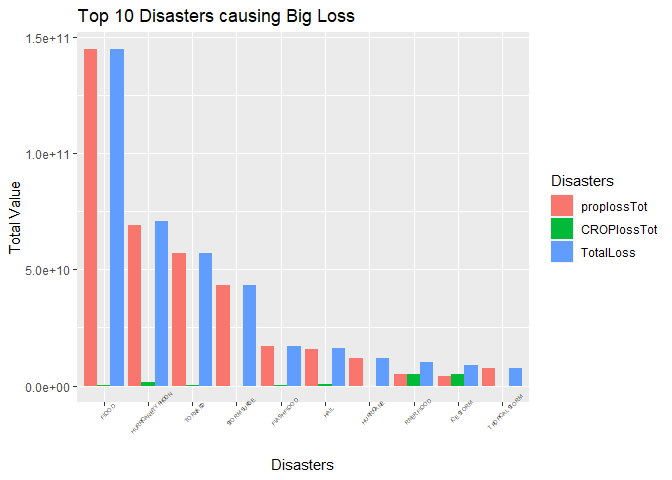
\includegraphics{FinalScript_files/figure-latex/unnamed-chunk-7-1.pdf}

\hypertarget{result-conclusion}{%
\subsection{Result / Conclusion}\label{result-conclusion}}

We see that tornadoes cause more fatalities and injuries in a rate that
is significantly greater than the rest of Disasters. Tornadoes are most
harmful to population health in this dataset.

it is obvious that Flood is the most destructive weather events for
economic consequences, as documented in the data.It's greatly impact
economic consequences compare others disasters.

\end{document}
